\chapter{Datasets}\label{ch:datasets}
\section{CHiME 4/5}
\subsection{Overview}
The CHiME-4 dataset is provided 
as part of the CHiME challenge\cite{chimechal,chimebase}.

The challenge is to build an ASR model
for multi-microphone devices being used
in various noisy environments.

Six microphones are mounted on a tablet
device and are recorded with a high-resolution
multi-track recorder. Besides those six 
microphones, an additional 
close-talking microphone is recorded by
another recording device, daisy-chained to the
multi-microphone recording device.

The close-talking microphone is referenced as
the clean speech channel.

\subsubsection{CHiME Recording Scenarios}
\begin{figure}[H]
    \centering
    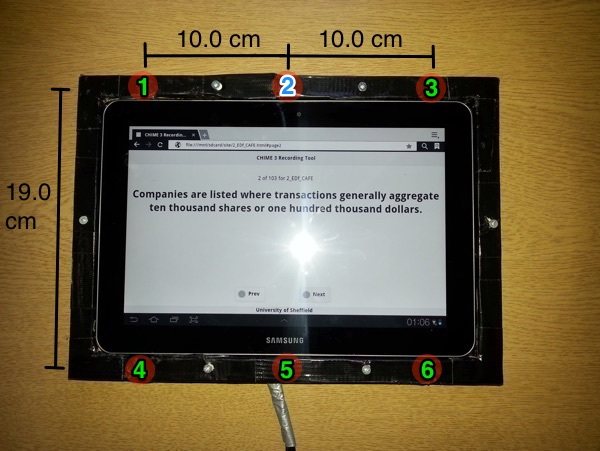
\includegraphics[width=0.75\linewidth]{Datasets/images/chime4_mic_array}
    \caption{CHiME-4 microphone-array}\label{fig:chime4_mic_array}
    \source{Adapted from \citep{Chime4Challenge}}
\end{figure}

\begin{figure}[H]
    \centering
    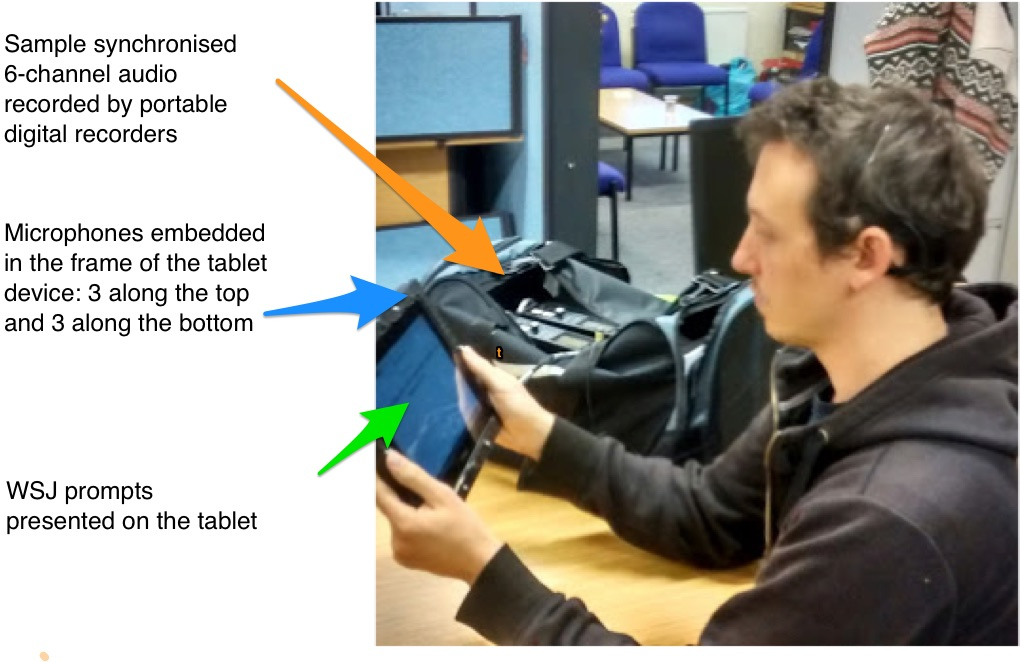
\includegraphics[width=0.75\linewidth]{Datasets/images/chime4_rec_device}
    \caption{CHiME-4 recording setup}\label{fig:chime4_rec_device}
    \source{Adapted from \citep{Chime4Challenge}}
\end{figure}

Four different noisy environments were selected, a Cafe, a street junction, a bus, and a pedestrian area.

The CHiME-4 dataset stats are shown in Figure Table\;\ref{fig:chime4_stats}

\begin{figure}[H]
    \centering
    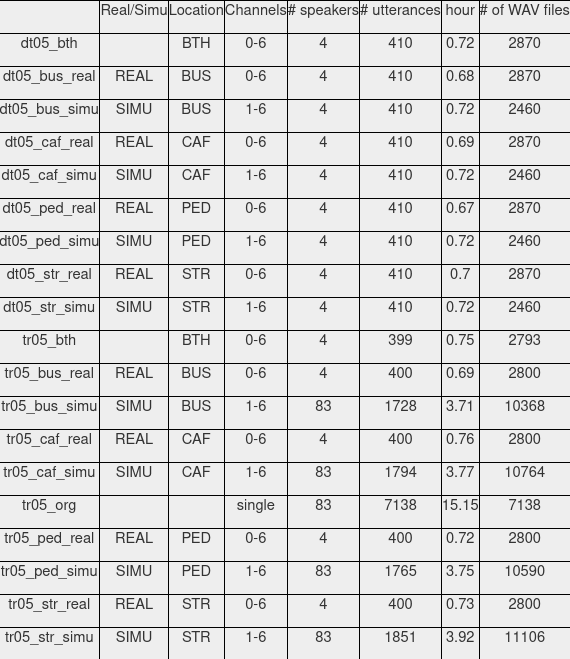
\includegraphics[width=0.75\linewidth]{Datasets/images/chime4_stats}
    \caption{CHiME-4 recording setup}\label{fig:chime4_stats}
    \source{Adapted from \citep{Chime4Challenge}}
\end{figure}


% \section{LibriSpeech}
% \subsection{Development}
% \subsection{Train}
% \subsection{Test}

\section{CommonVoice}
The CommonVoice dataset is an open-source, 
free dataset provided by Mozilla\cite{commonVoiceDS}.

CommonVoice for the English corpus
contains overall \(2886\) hours of recordings, where
\(2185\) hours of them were validated by the community.
\(79,398\) different voices construct the dataset.
\bigskip

Statistics and distributions for the CommonVoice dataset 
are shown in Table\;\ref{tbl:commvoice_stats}.

\begin{table}[H]
    % for more info see: https://www.overleaf.com/learn/latex/tables
    \centering
    % \hspace*{-2.8cm}
    \arrayrulecolor{ytblborder}
\begin{tabular}{ !{\color{ytblborder}\vrule}l!{\color{ytblborder}\vrule}l| } 
    \hline

    % \hline
    % \rowcolor{ytblcaption} \color{white}\bf{Parameter} 
    % & \color{white}\bf{Engine \#72} \\
    % % & \color{white}\bf{ORM} 
    % % & \color{white}\bf{Clean} \\
    % \hline

    % \hline\hline
    % \rowcolor{ytblcaption}\multicolumn{3}{|c|}{\bf{CNN Settings}}   \\
    % \hline

    \hline
    \cellcolor{ytbl} \multirow{10}{1em}{}
                            & \cellcolor{wtbl} 23\% United States English \\
    \cellcolor{ytbl}        & \cellcolor{wtbl} 8\% England English \\
    \cellcolor{ytbl}        & \cellcolor{wtbl} 7\% India and South Asia \\
    \cellcolor{ytbl}        & \cellcolor{wtbl} 3\% Canadian English \\
    \cellcolor{ytbl}        & \cellcolor{wtbl} 3\% Australian English \\
    \cellcolor{ytbl}Accent  & \cellcolor{wtbl} 2\% Scottish English \\
    \cellcolor{ytbl}        & \cellcolor{wtbl} 1\% New-Zealand English \\
    \cellcolor{ytbl}        & \cellcolor{wtbl} 1\% Southern African \\
    \cellcolor{ytbl}        & \cellcolor{wtbl} 1\% Irish English \\
    \cellcolor{ytbl}        & \cellcolor{wtbl} 51\% Undeclared \\
    \hline
    
    \hline
    \cellcolor{wtbl} \multirow{8}{1em}{}
                            & \cellcolor{wtbl} 24\% 19-29 \\
    \cellcolor{wtbl}        & \cellcolor{wtbl} 13\% 30-39 \\
    \cellcolor{wtbl}        & \cellcolor{wtbl} 10\% 40-49 \\
    \cellcolor{wtbl}        & \cellcolor{wtbl} 6\% <19 \\
    \cellcolor{wtbl}Age     & \cellcolor{wtbl} 4\% 60-69 \\
    \cellcolor{wtbl}        & \cellcolor{wtbl} 4\% 50-59 \\
    \cellcolor{wtbl}        & \cellcolor{wtbl} 1\% 70-79 \\
    \cellcolor{wtbl}        & \cellcolor{wtbl} 38\% Unknown \\
    \hline

    \hline
    \cellcolor{ytbl} \multirow{3}{1em}{}
                            & \cellcolor{wtbl} 45\% Male \\
    \cellcolor{ytbl}Gender  & \cellcolor{wtbl} 15\% Female \\
    \cellcolor{ytbl}        & \cellcolor{wtbl} 40\% Unknown \\
    \hline

    \hline
\end{tabular}
\arrayrulecolor{black}
\caption{CommonVoice dataset statistics}
\label{tbl:commvoice_stats}
\end{table}

During training, we dropped 
recordings longer than ten seconds.
This is because the dataset contains 
open-mic recordings, which cause the 
feature vector to be so large that 
it cannot fit in either the GPU's 
dedicated RAM or the server's memory.
As a result of omitting recordings longer than the ten seconds threshold, some recordings, although being valid, are still marked as open-mic and also dropped from the dataset.

\bigskip

Another issue we faced with the CommonVoice dataset is
that some recordings were not validated and thus could be corrupted.
Filtering out of those recordings is very cumbersome
and would take long a time to complete. 
Therefore, the number of
non-validated recordings participating in the training, 
validation, or testing phases had been cut to half. 
We have seen some performance degradation in terms of WER and CER
due to non-validated recordings in the test and validation 
measurements. However, these faulty measures are sparse
compared to the validated recordings measures, introducing
only a slight impact on the mean value, but can be seen
in the variance fluctuations presented in the bar plots
in Chapter\;\ref{ch:asr_ch}.

Table\;\ref{tbl:comvoice_set_dstrb} summarizes the CommonVoice
dataset subsets and the number of recordings each subset contains.

\begin{table}[H]
    % for more info see: https://www.overleaf.com/learn/latex/tables
    \centering
    \begin{tabular}{lr}
      \midrule
      Set & Utterances [\(N\)] \\
      \midrule
        Training    & 759,546   \\
        Dev/Valid   & 16,264   \\
        Test        & 16,236  \\
       \bottomrule
    \end{tabular}
    \caption{CommonVoice sets utterances distribution}\label{tbl:comvoice_set_dstrb}
\end{table}